\documentclass[a4paper,11pt]{article}
%\pdfoutput=1 % if your are submitting a pdflatex (i.e. if you have
%             % images in pdf, png or jpg format)

\usepackage{jcappub} % for details on the use of the package, please
                     % see the JCAP-author-manual
\usepackage{siunitx}
\usepackage[T1]{fontenc} % if needed
\usepackage{subcaption}

\title{Physical Characteristics Required of a Millisecond Pulsar Population to Reproduce the Galactic Center Excess}


%% %simple case: 2 authors, same institution
%% \author{A. Uthor}
%% \author{and A. Nother Author}
%% \affiliation{Institution,\\Address, Country}

\author{Jack Dinsmore}
\author{and Tracy Slatyer}
\affiliation{Massachusetts Institute of Technology \\Cambridge, MA, USA}

% e-mail addresses: one for each author, in the same order as the authors
\emailAdd{jtdinsmo@mit.edu}
\emailAdd{tslatyer@mit.edu}

\newcommand{\parens}[1]{\left(#1\right)}
\newcommand{\brackets}[1]{\left[#1\right]}
\newcommand{\expp}[1]{\exp \parens{#1}}
\newcommand{\fraci}[2]{#1 / #2}
\newcommand{\comment}[1]{\emph{\color{red}{#1}}}

\DeclareSIUnit\erg{erg}
\DeclareSIUnit\parsec{pc}
\DeclareSIUnit\photon{photon}
\newcommand{\SIasym}[4]{#1^{+#2}_{-#3}\ \SI{}{#4}}% Asymmetric error bars
\newcommand{\numasym}[3]{#1^{+#2}_{-#3}}% Asymmetric error bars



\abstract{An excess of gamma rays emanating from the Galactic Center has been discovered and proven to be robust. One proposed solution is the presence of a large number of unresolved millisecond pulsars in the Galactic Center. We analyze the number of pulsars required for such a population to reproduce the GCE, and compare the predicted number of resolvable pulsars and the amount and distribution of flux emitted by those resolvable pulsars to observations. We predicate these calculations on luminosity functions discussed in literature and demonstrate which luminosity functions are excluded by observations. We conclude with an analysis of the capacity of future increases in observational sensitivity to rule out more luminosity functions.}



\begin{document}
\maketitle
\flushbottom



\section{Introduction}
\comment{What is the GCE?}\cite{Goodenough:2009gk}

\comment{What are possible explanations for the GCE? DM or MSPs. What luminosity functions might they have? Mention that the GCE MSP population must be distinct from the disk population, and that accretion induced collapse yields different MSPs than other birth processes.}

\comment{Mention Fermilab's paper, the 3 M pulsar population.}

\comment{Data sources}

\comment{The specific luminosity function parameterizations we use correspond to parameterizations that are reasonable for an MSP explanation to the GCE. But a lot of this analysis, such as the plots of allowed parameterizations for the power law and log normal luminosity functions, simply model point source emission, not necessarily MSPs. Is it useful to make this distinction?}

In this paper, we extract a total flux for the GCE drawn from other analyses, and use it to calculate the total number of pulsars, number of resolved pulsars, and flux from those resolvable pulsars as predicted by various luminosity functions that have been proposed in literature. Making use of three different models for the sensitivity of \textit{Fermi}, we indicate the luminosity function parameterizations necessary in order to meet the observational constraints imposed by a point source template fit to \textit{Fermi} data and the 4FGL catalog. We operate under the assumption that every resolved point source is an MSP and the GCE consists entirely of MSPs.

After comparing the observed flux distribution of point sources in the GCE to the MSP flux distribution predicted by these luminosity functions, we then discuss how many MSPs are likely to make up the GCE under these assumptions, given the observational constraints. We conclude with an analysis of what further luminosity function constraints could be achieved by improvements to the sensitivity of \textit{Fermi}.


\section{Methods \& Datasets}
\subsection{GCE Spacial distribution}
We model the spacial distribution of MSPs in the GC with an NFW squared profile, to match with empirical data. The number density of an NFW profile is spherically symmetric, with radial density profile
\label{sec:spacial-distro}
\begin{equation}
    \rho_\text{NFW}(r) \propto \parens{\frac{r}{r_s}}^{-\gamma}\parens{1 + \frac{r}{r_s}}^{-3+\gamma}
    \label{eqn:nfw}
\end{equation}
where $\gamma = 1.2$ and $r_s = \SI{20}{\kilo\parsec}$ for this work. Other sources occasionally use $\gamma = 1$.

We allow this NFW distribution to extend over a region of interest (ROI) extending within $|\ell| < 20^\circ$ and $2^\circ < |b| < 20^\circ$, where we have cut out the Galactic disk. We also restrict the luminosity of the GCE to within $\SI{0.1}{\giga\electronvolt} < E_\gamma < \SI{100}{\giga\electronvolt}$. Both these ranges are slightly on the wider side of those commonly used in literature.


\subsection{Observables}
\label{sec:observables}
To fit the luminosity functions described in section \ref{sec:lum-funcs}, we will use three observables: the total flux of the GCE $F_\text{GCE}$, the ratio of the total flux to the flux visible from point sources resolved by \textit{Fermi} $R_\text{r}$, and the number of resolved point sources $N_\text{r}$. The first observable, $F_\text{GCE}$, is described in section \ref{sec:total-lum}, but we describe the other two observables in this section.

$N_\text{r}$ and $R_\text{r}$ have been studied by \comment{Some technical name for the Fermilab team.} \cite{Zhong:2019ycb}. The authors performed a template fit to data from Fermi-LAT to isolate spacial peaks in flux, finding 107 unique peaks within 0.3$^\circ$ of a source in the 4FGL catalog within the region of interest \cite{Abdollahi_2020}. Of these sources, they exclude all that are listed in the 4FGL catalog as not associated with pulsars. Of those that are known to be pulsars, they exclude all whose positions are known not to be within $\SI{2}{\kilo\parsec}$ of the GC via the ATNF Pulsar Catalog \cite{Hobbs04}. This leaves 47 point sources in the 4FGL catalog whose origins are either known to be pulsars in the GC or are unknown. We will therefore set $N_\text{r} = 47$ for this paper. If the allowed distance between a flux peak and a 4FGL source is extended from 0.3$^\circ$ to $0.55^\circ$, five more sources are added. Together, the 47 sources are responsible for $R_\text{r}=0.2$ of the total GCE flux. \comment{Shouldn't I actually redo this addition given the fact that I'm now not using the same GCE flux as Fermilab?} These 47+5 sources used here are displayed in figure \ref{fig:47-sources}.

\begin{figure}
    \centering
    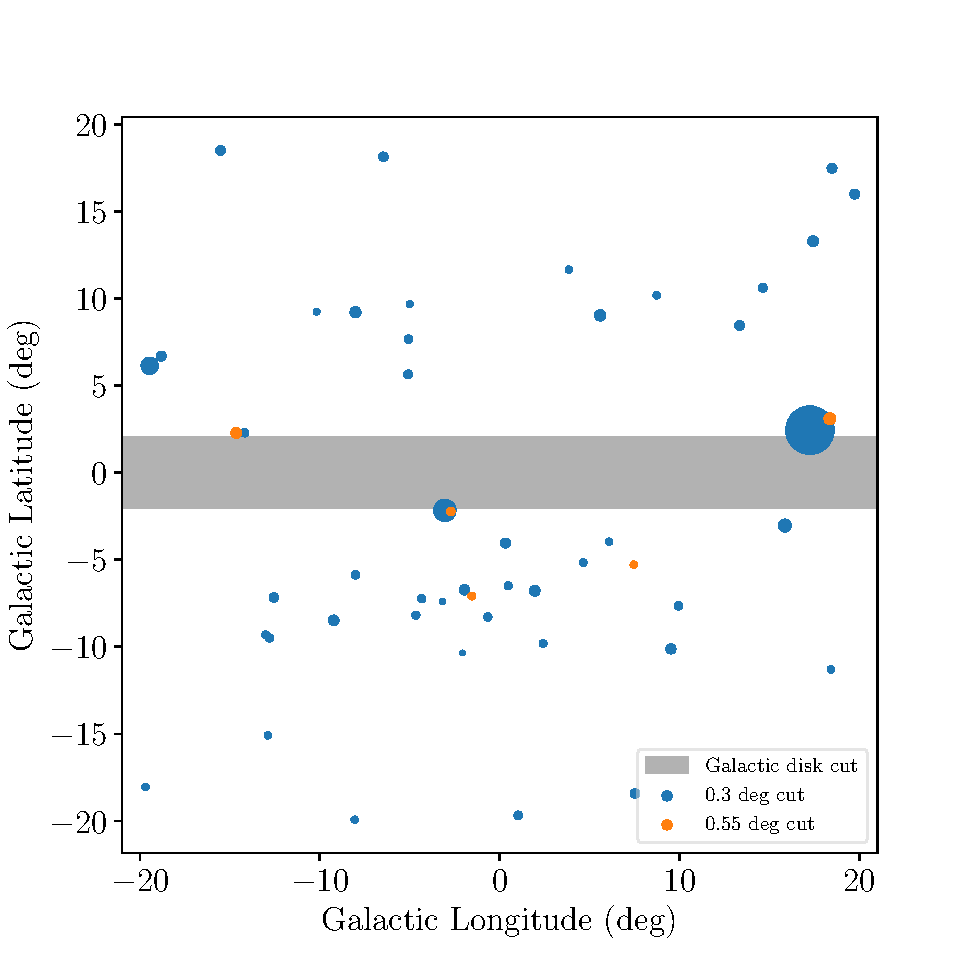
\includegraphics[width=0.5\textwidth]{figs/point-source-positions.pdf}
    \caption{The 47 point sources within $0.3^\circ$ of a 4FGL source. Also shown are the 5 sourecs added by extending to $0.55^\circ$ separation. The sources are scaled by luminosity in radius. The gray band represents the $|b| \leq 2^\circ$ cut made around the galactic disk. \comment{I think this disagrees with the Fermilab paper}}
    \label{fig:47-sources}
\end{figure}

It is important to note that the above values for $N_\text{r}$ and $R_\text{r}$ define an allowed region, which includes populations with lower $N_\text{r}$ and $R_\text{r}$, because some of the unknown sources might not be pulsars.



We will also discuss a third feature of a potential MSP population in the GC: the total number of MSPs $N_\text{GCE}$, resolved or unresolved. This number is not measurable, but serves as a useful reference to gauge the physicality of any population of MSPs. \comment{Mention that it's expected to be around 40,000.}


\subsection{Total GCE Luminosity}
\label{sec:total-lum}
An estimate of the total flux of the GCE is necessary for our study, so we extract the total flux from several previous analyses of spectra using the following three methods and compare them. The spectral analyses we study here are refs. \cite{Zhong:2019ycb, Calore:2014xka, DiMauro:2021raz, Abazajian:2014fta, Gordon13, Ajello:2015kwa}. Although they take their data from the same source, \textit{Fermi}, the studies' spectra differ due to choices in the method of fitting. For example, to model the spacial distribution of the excess, refs. \cite{Calore:2014xka, Gordon13, Ajello:2015kwa} fix $\gamma=1.2$, while ref. \cite{Zhong:2019ycb} performs the analysis for both $\gamma=1.0$ and $\gamma=1.2$, and refs. \cite{DiMauro:2021raz, Abazajian:2014fta} allow $\gamma$ to arise out of the fit. For the cases in which $\gamma$ is fitted, typical valyes range in 1.1--1.3.

The studies use ROIs ranging from a $40^\circ \times 40^\circ$ region without the galactic disk cut used in this paper, to a $7^\circ \times 7^\circ$ region. All ROIs are centered on $(\ell, b)=(0, 0)$, however. All studies fix $r_s=\SI{20}{\kilo\parsec}$, except for refs. \cite{Abazajian:2014fta, Gordon13}, which use $r_s=\SI{23.1}{\kilo\parsec}$. In order to compare the studies, we rescale ROIs by the process described in appendix \ref{app:roi-rescale}, but we do not correct for differences in $\gamma$ or $r_s$.

The manner in which uncertainties are reported also varies; some studies report only statistical uncertainties, and some report both statistical and systematic. Refs. \cite{Calore:2014xka, Gordon13} report both separately, and for our purposes we add these in quadrature.

Figure \ref{fig:all-spectra} displays all the spectra mentioned above, with ROI rescaling included. When error bars can be recovered from the original papers, they are displayed. Many studies reported flux values in units of flux per steradian; we have multiplied those fluxes by the area of their respective ROIs to attain an absolute value for the GCE spectrum.

\begin{figure}
    \centering
    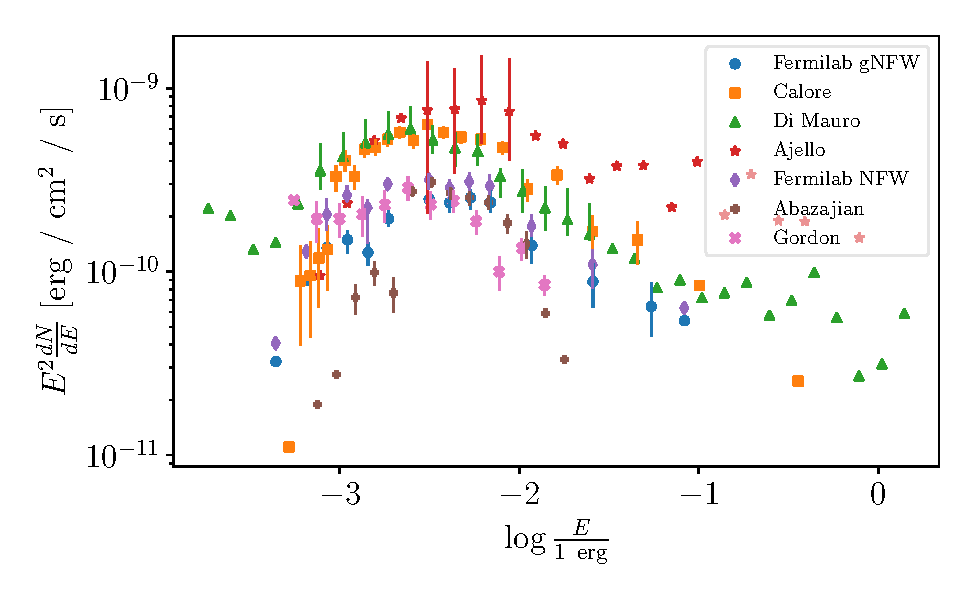
\includegraphics[width=0.7\textwidth]{figs/all-spectra.pdf}
    \caption{Spectra from seven analyses of the GCE, using different background models, shown with error bars when reported.}
    \label{fig:all-spectra}
\end{figure}

We use compare three methods of extracting the total GCE flux from these spectrum analyses. The first method is direct numerical integration of the spectra provided by each source. This method is most sensitive to the data measured by \textit{Fermi} and does not attempt to abstract over it with a smooth function, but it is only available where points are reported, and is most sensitive to experimental error. Therefore, we also consider a broken law fit to the data, of the same form as the NPTF luminosity function: eq. \ref{eqn:nptf}. It has four parameters: a constant of proportionality, the turnover energy $E_\text{b}$, and the slopes above and below the turnover flux $n_2$ and $n_1$. This function can then be analytically integrated over all flux values to get the total flux of the GCE. Many of the analyses cited above only report error bars on some points, because error bars on the other points are too large. We therefore fit only to the points with error bars reported.

Unfortunately, for some analyses, the number of points reported with error bars is only slightly larger than the number of parameters of the broken power law function. To ensure that the fit result is less prone to statistical deviations of a small number of points, we use a third method in addition to the above two. Ref. \cite{Calore:2014xka} provides broken power law fit parameters for their GCE flux spectral data: $F_\text{b} = \SIasym{2.06}{0.23}{0.17}{\giga\electronvolt}$. $n_1 = \numasym{1.42}{0.22}{0.31}$, $n_2 = \numasym{2.63}{0.13}{0.095}$. The third fitting method is to fix these three broken power law parameters at these values and allow only the overall normalization to vary. An example of all three of these fitting methods applied to reference \cite{DiMauro:2021raz} and shown in figure \ref{fig:di-mauro-example}.

\begin{figure}
    \centering
    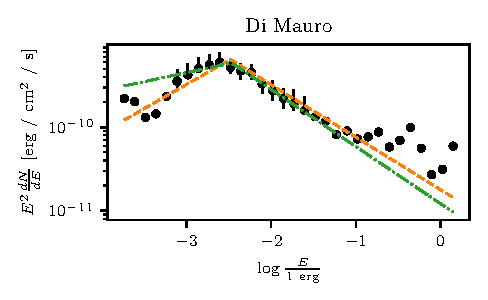
\includegraphics[width=0.7\textwidth]{figs/di-mauro-example.pdf}
    \caption{Spectrum produced by di Mauro in ref. \cite{DiMauro:2021raz}, with the two broken power law models fitted and shown.}
    \label{fig:di-mauro-example}
\end{figure}

In practice, the numerical integration method appears to yield lower flux values, because it does not extend the tails of the spectrum. However, the two power law fits usually result in similar values for a single analysis. However, the values provided by different analyses vary greatly. For this study, we use the value obtained from di Mauro's analysis because it occupies a position near the middle of the distribution of GCE luminosities \comment{(Not anymore!)} and is a recent study. We choose the value obtained by numerical integration, which was $F_\text{GCE} = \SI{1.295e-9}{\erg\per\centi\meter\squared\per\second}$.

\begin{figure}
    \centering
    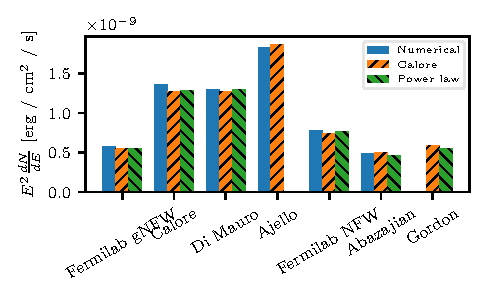
\includegraphics[width=0.8\textwidth]{figs/total-flux-bars.pdf}
    \caption{Total flux of the GCE as determined by the three integration methods discussed.}
    \label{fig:total-flux-bars}
\end{figure}

\subsection{Luminosity Functions}
\label{sec:lum-funcs}
Previous work has modeled the GCE as a MSP population, and estimated the probability distribution of pulsar luminosities, termed the ``luminosity function.'' One such luminosity function, proposed by ref. \cite{Zhong:2019ycb} among others, is an exponentially damped power law:
\begin{equation}
    P_\text{Power law}(L) = L^{-\alpha} \expp{-\frac{L}{L_\text{max}}}\brackets{\Gamma\parens{1-\alpha, \frac{L_\text{min}}{L_\text{max}}}L_\text{max}^{1-\alpha}}^{-1}.
    \label{eqn:power-law}
\end{equation}
This luminosity function restricts the range of luminosities to $[L_\text{min}, \infty)$, where $L_\text{min}$, $L_\text{max}$, and $\alpha$ are free parameters. \comment{The following should probably be moved to the introduction once I write it, where Fermilab's research is described.} This reference found that $(\SI{1e29}{\erg\per\second}$, $ \SI{1e35}{\erg\per\second}$, $1.94)$ is required reproduced observations. They find that this model admits three million MSPs in the GCE, which differs from estimates based on the physical properties of observed MSPs that estimate the number of MSPs at the Galactic center at the order of 40,000 \cite{citation_needed}.

Ref. \cite{osti_1305131} proposes a power law luminosity function of
\begin{equation}
    P_\text{Log normal}(L)= \frac{\log_{10} e}{\sigma \sqrt{2\pi} L}\expp{-\frac{\parens{\log_{10} L - \log_{10} L_0}^2}{2\sigma^2}},
    \label{eqn:log-normal}
\end{equation}
where $L_0$ and $\sigma$ are free parameters. The ref. fits this model to data from globular cluster (GCL) MSP populations, yielding values $L_0 = \SI{8.8e33}{\erg\per\second}$ and $\sigma=0.62$. It predicts thousands of MSPs to occupy the GCE if the entire excess is to be explained by MSPs.

Ref. \cite{Ploeg:2020jeh} proposes a more intricate luminosity function, derived from a model of the pulsars themselves. They find that differences in spectrum between resolved, globular cluster MSPs in the Galactic disk and unresolved MSPs at the Galactic center are not significant. Their luminosity function generated for the galactic disk closely resembles a log normal luminosity function as in equation, where $L_0 = \SI{1.61e+32}{\erg\per\second}$ and $\sigma=0.700$ were obtained from a least-squares fit with $p$-value very close to 1.

Another study by Gautam et al. analyzes the possibility that the hypothetical MSP population in the GCE is generated not by the Low Mass X-Ray Binary formation, but by Accretion Induced Collapse \cite{Gautam:2021wqn}. \comment{To distinguish between this, a definition of these two collapse methods, along with models other than an MSP model, should be put in the introduction. Mention the fact that the MSPs in the GCE would have to look different from that in the disk.} Their binary system model yields a numerical luminosity function for MSPs in the GC, reported as a function of flux. Converting to luminosity in the manner described in appendix \ref{app:lum-to-flux}, we perform a least-squares fit of a log normal distribution to their function, which produces $L_0 = \SI{3.92e+32}{\erg\per\second}$ and $\sigma = 0.937$, with a $p$-value of 0.29. We call this model the AIC log normal model.

Finally, ref. \cite{Lee:2015fea} proposes a broken-power law luminosity function of
\begin{equation}
    P_\text{NPTF}(L) = \parens{\frac{\parens{1-n_1}\parens{1-n_2}}{L_b \parens{n_1 - n_2}}}\begin{cases}
        \parens{\fraci{L}{L_\text{b}}}^{-n_{1}} & L < L_{b} \\
        \parens{\fraci{L}{L_\text{b}}}^{-n_{2}} & L > L_b
    \end{cases}
    \label{eqn:nptf}
\end{equation},
where the free parameters  $n_1$, $n_2$, and $L_b$ were found via a Non-Poissonian Template Fitting model (NPTF) to be $(18.2, -0.66, \SI{9.13e+33}{\erg\per\second})$ for an NFW-squared-distributed population of MSPs named NFW PS. The paper proposes a second luminosity function named Disk PS with parameters $(17.5, 1.4, \SI{3.53e+35}{\erg\per\second})$, which is unnormalizable except when a minimum luminosity of pulsars $L_\text{min}$ is introduced. The luminosity-valued parameters were originally given as fluxes in $\SI{}{\photon \per \centi\meter\squared \per \second}$. The photon energy was calculated via appendix \ref{app:photon-energy} and the flux converted to luminosity via appendix \ref{app:lum-to-flux}.

We set $L_\text{min}=\SI{1e29}{\erg\per\second}$, which is the same minimum pulsar luminosity used by ref. \cite{Zhong:2019ycb}. The turnover luminosity $L_\text{b}$ was given as a photon flux value in units of photons per centimeter squared per second; the process used to convert from photon flux to luminosity is detailed in the methods section.

All the above-mentioned luminosity functions are shown in figure \ref{fig:lum-funcs}.

\begin{figure}
    \centering
    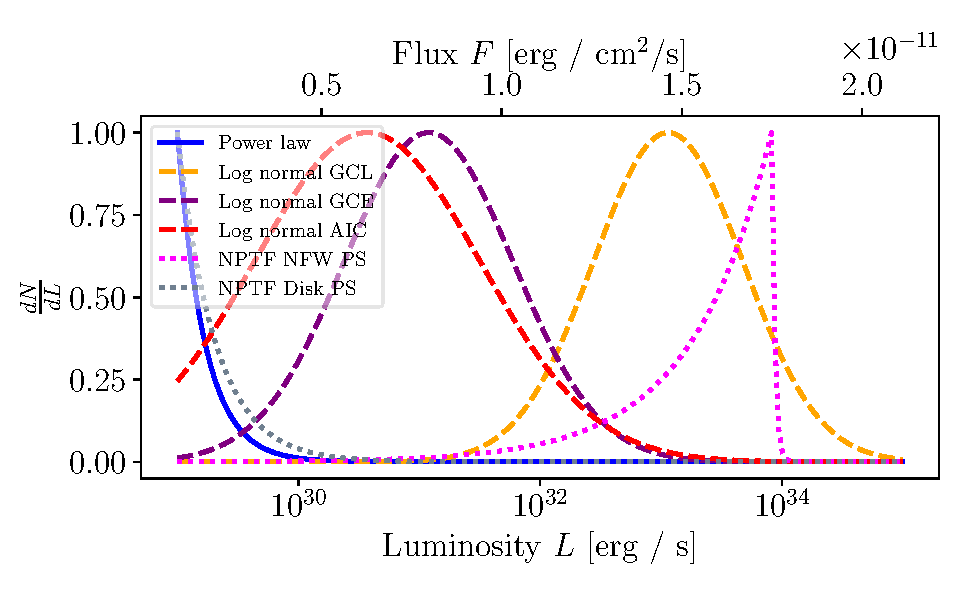
\includegraphics[width=0.49\textwidth]{figs/lum-funcs.pdf}
    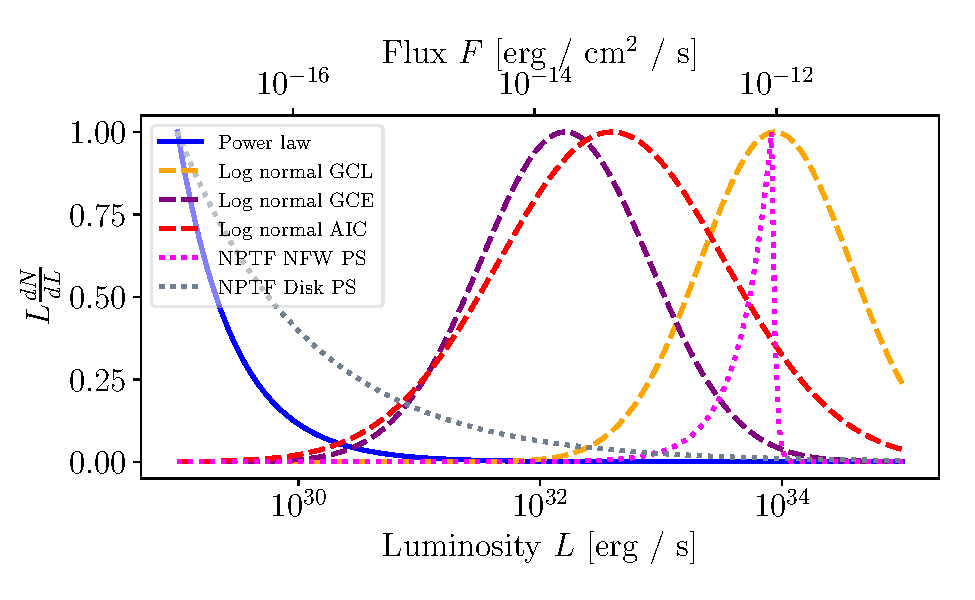
\includegraphics[width=0.49\textwidth]{figs/l-lum-funcs.pdf}
    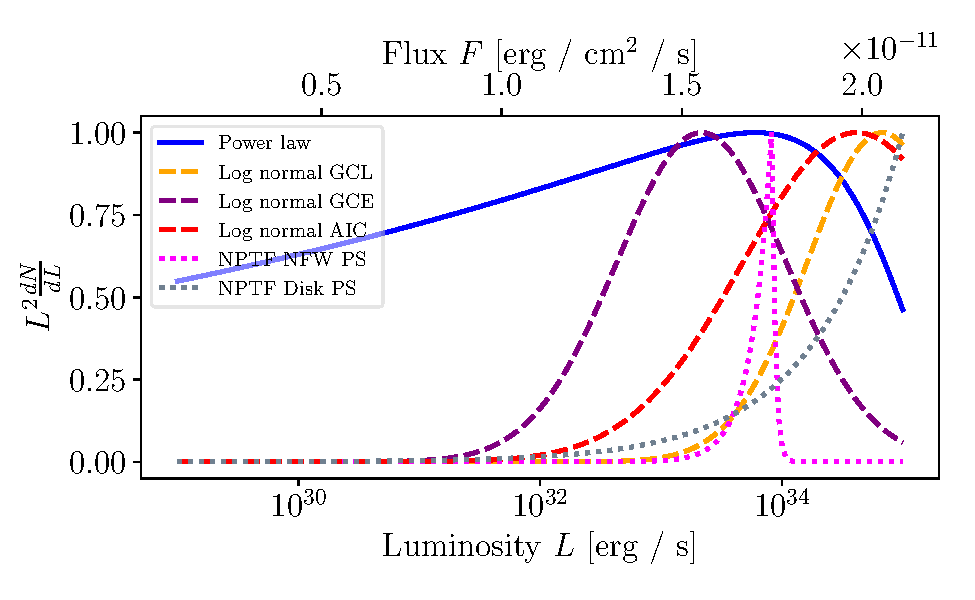
\includegraphics[width=0.49\textwidth]{figs/l2-lum-funcs.pdf}
    \caption{\textit{Left:} Power law, GCL log normal, GCE log normal, and NPTF luminosity functions for MSPs in the GCE, vertically rescaled. \textit{Right:} Same plot as \textit{left} but weighted by luminosity. \textit{Bottom:} Same plot as above two but weighted by luminosity squared.}
    \label{fig:lum-funcs}
\end{figure}


\subsection{Sensitivity Models}
\label{sec:sensitivity}
The \textit{Fermi} telescope does not detect every pulsar in the GC; background emission obscures dimmer pulsars, and statistical effects cause some brighter sources to be unresolved. We make use of three sensitivity models to account for these factors.

The first, and simplest, is a step function luminosity model. It asserts that all point sources with $L>L_\text{th}$ are resolved, and none with $L<L_{\text{th}}$. Here, $L_\text{th} = \SI{e34}{\erg\per\second}$. This sensitivity model is the one used by ref. \cite{Zhong:2019ycb} to obtain the parameters of the power law luminosity function described in the paragraph after eq. \ref{eqn:power-law}. The four properties we intend to measure are then given by
\begin{equation}
    \begin{split}
        L_\text{GCE} &= N_\text{GCE}\int_{L_\text{min}}^\infty L P(L) dL \,, \qquad
        L_\text{r} = N_\text{GCE}\int_{L_\text{th}}^\infty L P(L) dL \,, \\
        N_\text{r} &= N_\text{GCE}\int_{L_\text{th}}^\infty P(L) dL \,,
        \label{eqn:observables-sens-1}
    \end{split}
\end{equation}
where $N_\text{GCE}$ is a normalization constant, fixed by requiring that the luminosity of the GCE $L_\text{GCE}$ reproduces the flux $F_\text{GCE}$ observed. The conversion between $L_\text{GCE}$ and $F_\text{GCE}$ required to force this equivalence is outlined in appendix \ref{app:lum-to-flux}.

The second sensitivity model acknowledges the effect of background flux on resolvability and uses a position-dependent flux threshold $F_\text{th}(b, l)$ published by the \textit{Fermi} team \cite{Fermi-LAT:2019yla, Ballet:2020hze} (figure \ref{fig:sensitivity}). \comment{Here, I could assess how accurate 1e34 ergs/s actually is. One way would be simply to average over all the pixels in the sensitivity map and convert to luminosity. But isn't it better to weight the average by NFW distribution? In that case, I have to do a line of sight integral too, which means I can no longer use the flux to luminosity ratio in the appendix. It gets complicated...}. To calculate the four properties of GC MSP populations, we use
\begin{equation}
    \begin{split}
        F_\text{GCE} &= \int_\Omega d\Omega \int_0^\infty s^2 ds A \rho_{NFW}^2(r)\int_{L_\text{min}}^\infty dL \frac{L}{4\pi s^2}P(L)\,, \\
        N_\text{GCE} &= \int_\Omega d\Omega \int_0^\infty s^2 ds A \rho_{NFW}^2(r)\,, \\
        F_\text{r} &= \int_\Omega d\Omega \int_0^\infty s^2 ds A \rho_{NFW}^2(r)\int_{4\pi s^2F_\text{th}(\ell, b)}^\infty dL \frac{L}{4\pi s^2}P(L)\,, \\
        N_\text{r} &= \int_\Omega d\Omega \int_0^\infty s^2 ds A \rho_{NFW}^2(r)\int_{4\pi s^2F_\text{th}(\ell, b)}^\infty dL P(L) \,. \\
        \label{eqn:observables-sens-2}
    \end{split}
\end{equation}
Here, $\Omega$ represents the $20^\circ \times 20^\circ$ region of interest with $|b| < 2^\circ$ cut out, and $A$ is the coefficient of equation \ref{eqn:nfw}, fixed by forcing $F_\text{GCE}$ to equal the observed value. In equation \ref{eqn:observables-sens-2} represents the distance to the galactic center from the point of integration, and is determined by the law of cosines: $r^2 = s^2 + r_c^2 - 2r_c s \cos b \cos \ell$.

\begin{figure}
    \centering
    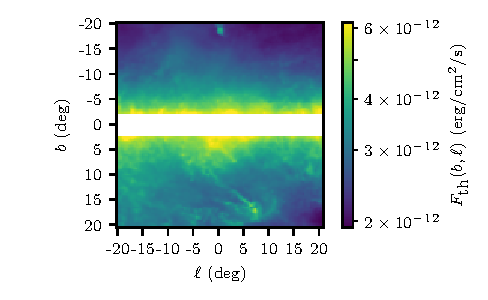
\includegraphics[width=0.7\textwidth]{figs/sensitivity-map.pdf}
    \caption{Position-dependent flux thresholds required to resolve an MSP, published by refs. \cite{Fermi-LAT:2019yla, Ballet:2020hze}. \comment{Maybe I shouldn't show this plot. It's not original; just a display of a FITS file pulled from the 4FGL website. But I could overlay the previous figure of where the 47 point sources are. Would that be useful?}}
    \label{fig:sensitivity}
\end{figure}

The third and final sensitivity model takes into account the statistical fluctuation of photons from point sources. Ref. \cite{Ploeg:2020jeh} models the probability that a point source with average flux $F$ is resolved as
\begin{equation}
    P_\text{r}(F) = \frac{1}{2} \parens{1 + \text{erf} \parens{\frac{\log_{10} F - (\log_{10} F_\text{th}(\ell, b) + K_\text{th})}{\sqrt{2}\sigma_\text{th}}}}
    \label{eqn:ploeg-smoothing}
\end{equation}
where $K_\text{th} = 0.45$ and $\sigma_\text{th} = 0.28$ were determined via an MCMC fit to globular cluster MSPs. The observables are calculated simply by multiplying the integrand of the luminosity integral in equation \ref{eqn:observables-sens-2} by $P_r(L/4\pi s^2)$ for $F_\text{r}$ and $N_\text{r}$. (Not for $F_\text{GCE}$, because we do not require that the $F_\text{GCE}$ flux be resolved.) \comment{Should I mention how much the sensitivity models differ, or wait until the results have been presented?}






\section{Results}
\subsection{$N_\text{r}$, $R_\text{r}$, and $N_\text{GCE}$ for different luminosity functions}
Using each of the luminosity functions outlined in section \ref{sec:sensitivity}, we extract the total number of resolvable MSPs $N_\text{r}$, the ratio of the flux received from those resolved MSPs to the total flux of the GCE $R_\text{r}$, and the total number of MSPs $N_\text{GCE}$ by forcing each function to reproduce the observed flux of the GCE. This is done for many parameterizations of the power law and log normal luminosity functions (eqs. \ref{eqn:power-law} and \ref{eqn:log-normal}), with $N_\text{GCE}$ displayed as a contour map in figures \ref{fig:step-function} and \ref{fig:position-dependent}, using the step function and the position-dependent sensitivity models respectively. The first row of these figures varies $L_\text{min}$ and $L_\text{max}$, with $\alpha=1.94$, which is the value computed by ref. \cite{Zhong:2019ycb}; the second row varies $L_\text{max}$ and $\alpha$, with $L_\text{min}=\SI{1e29}{\erg\per\second}$. The observations $N_\text{r}=47$ and $R_\text{r}=0.2$ trace out a one-parameter family of luminosity functions that is also displayed. Since some resolved sources may not in fact be part of the GC, the regions with $N_\text{r} < 47$ and $R_\text{r} < 0.2$ also satisfy observational constraints and are marked.

\begin{figure}
    \centering
    \begin{subfigure}[b]{0.49\textwidth}
        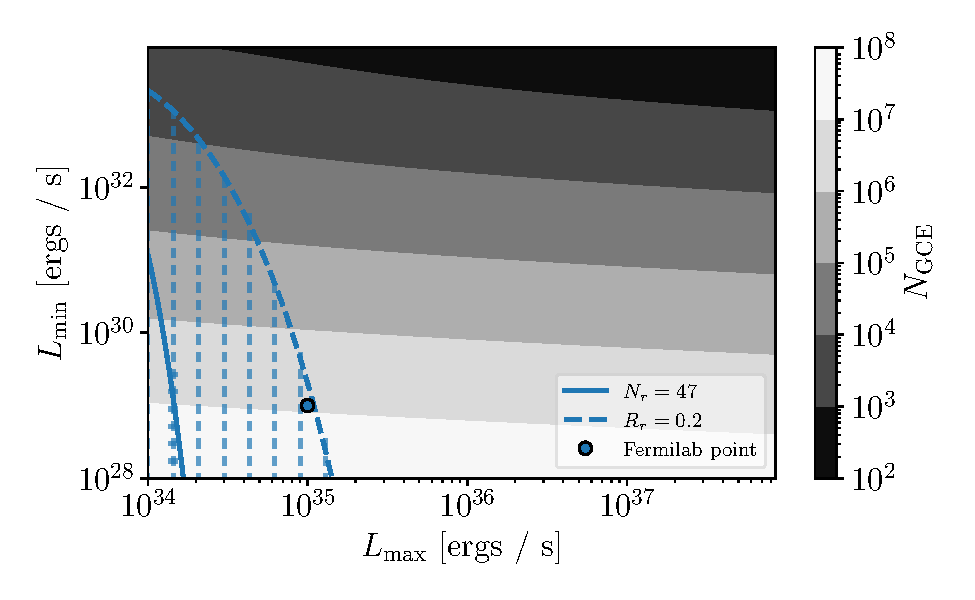
\includegraphics[width=\textwidth]{figs/power-law-step.pdf}
        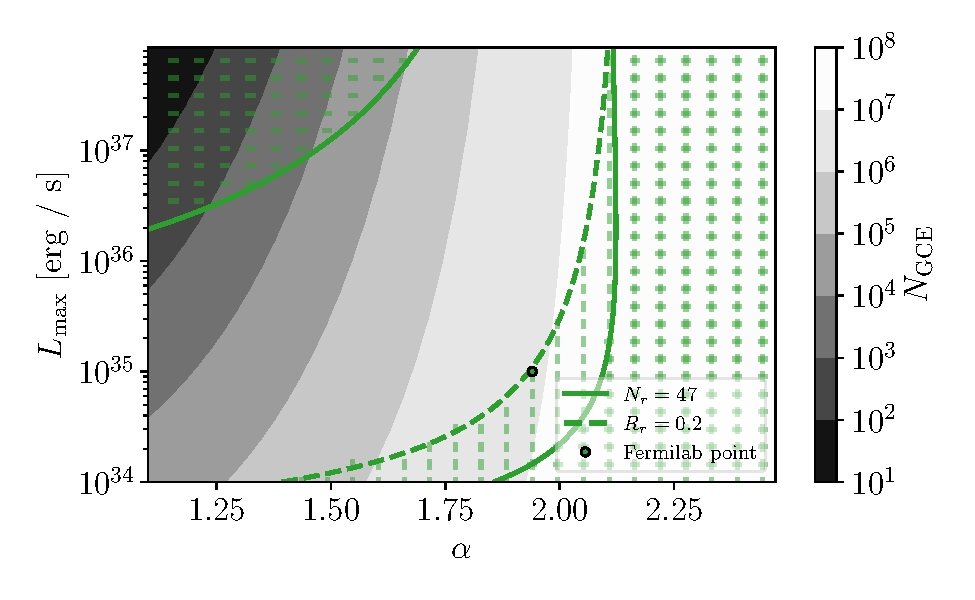
\includegraphics[width=\textwidth]{figs/power-law-alpha-step.pdf}
        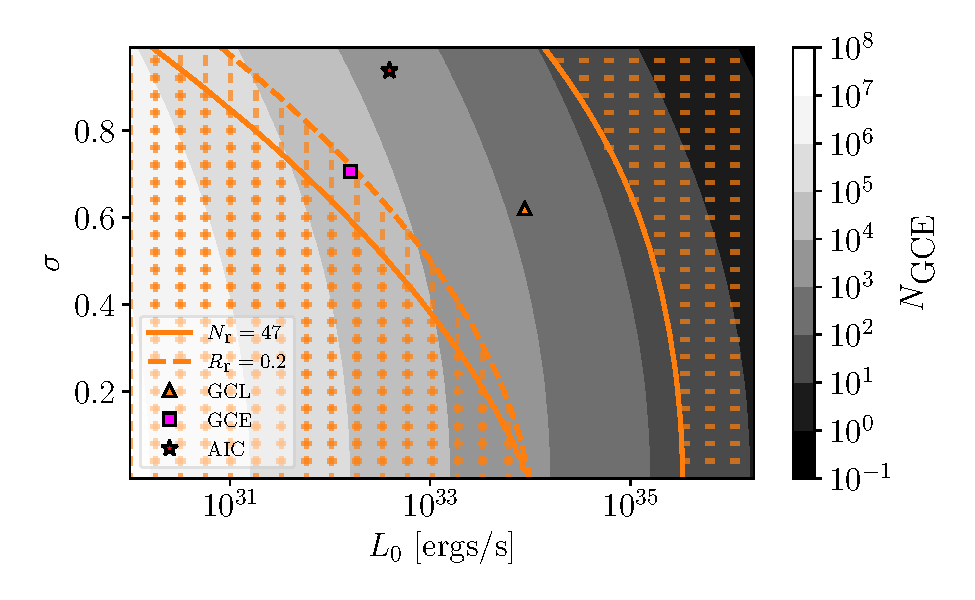
\includegraphics[width=\textwidth]{figs/log-normal-step.pdf}
        \caption{Step function sensitivity model}
        \label{fig:step-function}
    \end{subfigure}
    \hfill
    \begin{subfigure}[b]{0.49\textwidth}
        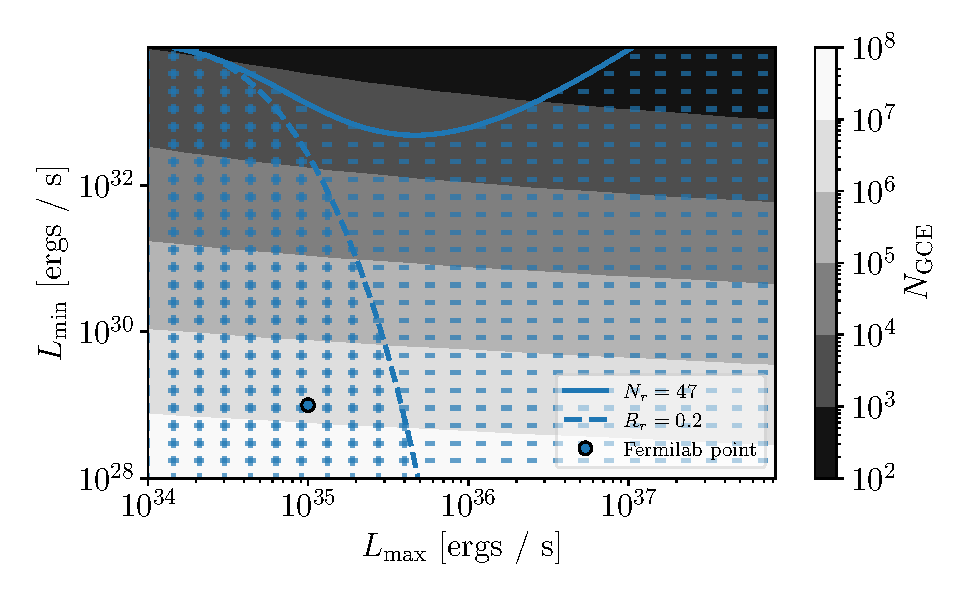
\includegraphics[width=\textwidth]{figs/power-law-pos-1x.pdf}
        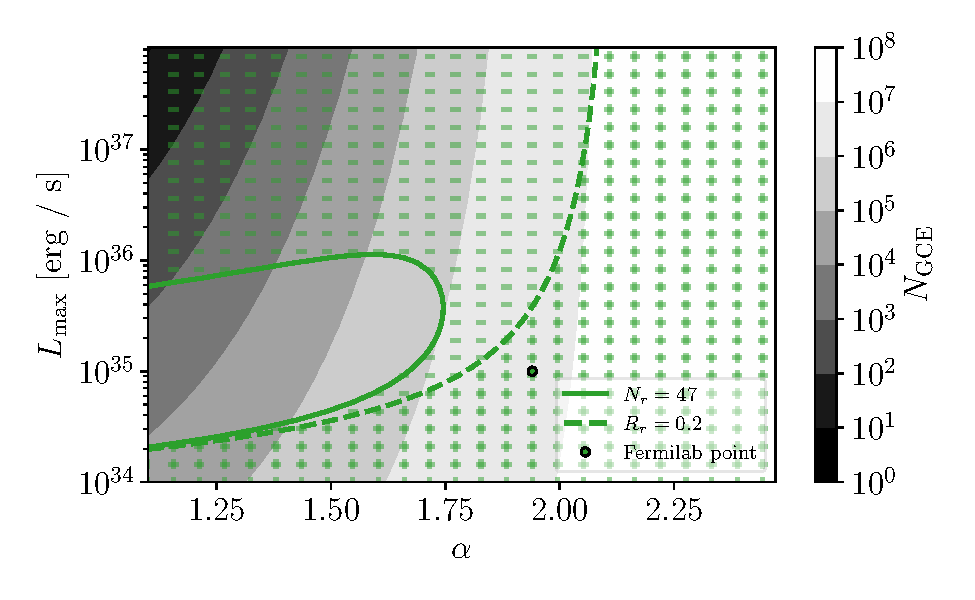
\includegraphics[width=\textwidth]{figs/power-law-alpha-pos-1x.pdf}
        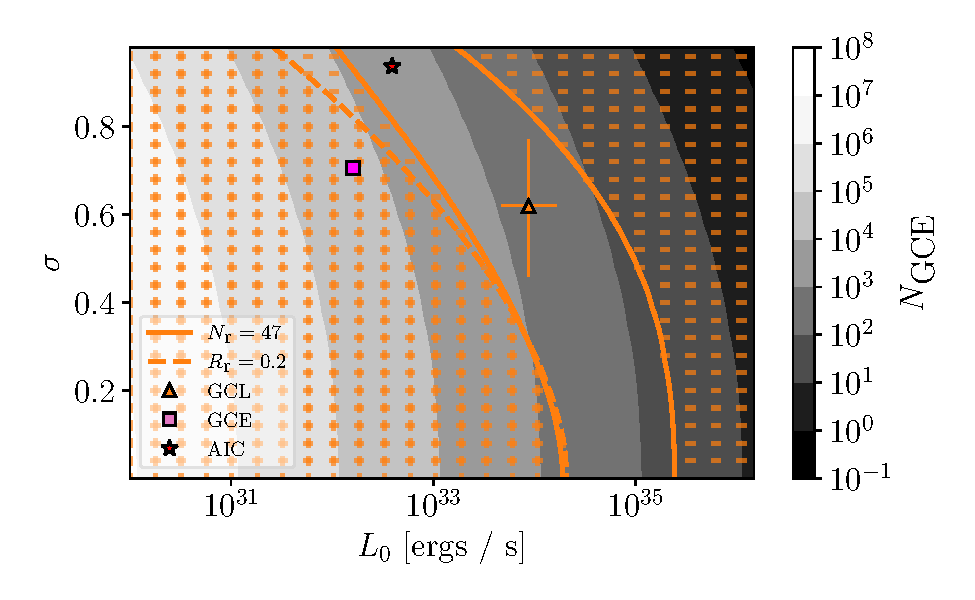
\includegraphics[width=\textwidth]{figs/log-normal-pos-1x.pdf}
        \caption{Position dependent sensitivity model}
        \label{fig:position-dependent}
    \end{subfigure}
    \caption{$N_\text{r}$, $R_\text{r}$, and $N_\text{GCE}$ calculations generated for parameterizations of a power law luminosity function (top two plots) and log normal (bottom plots). The parameterizations used in other analyses are marked. Regions allowed by the $N_\text{r} \leq 47$ and $R_\text{r} \leq 0.2$ are marked with \texttt{|} and \texttt{-} respectively, while regions allowed by both constraints are marked with \texttt{+}. The top power law plot (blue) fixes $\alpha=1.94$ while the lower (green) fixes $L_\text{min}=\SI{1e29}{erg\per\second}$.}
    \label{fig:step-and-pos}
\end{figure}

The analysis is also performed on the NPTF luminosity function, but only for the parameterization outlined in ref. \cite{Lee:2015fea} and therefore no figure is generated. Predictions for $N_\text{r}$, $R_\text{r}$, and $N_\text{GCE}$ for the specific parameterizations suggested by previous works are shown in table \ref{tab:specific-results} for all three sensitivity models.

\begin{table}
    \centering
    \begin{subtable}[h]{\textwidth}
        \centering
        \begin{tabular}{|p{4cm} >{\centering\arraybackslash}p{2cm} >{\centering\arraybackslash}p{2cm} >{\centering\arraybackslash}p{2cm}|}
            \hline
            Luminosity function & $N_\text{r}$ & $R_\text{r}$ & $N_\text{GCE}$\\ \hline \hline
            \textbf{Observation} & \textbf{47} & \textbf{0.2} & \\
            Power law & 115 & 0.193 & $\num{8.14e6}$ \\
            Log normal, GCL & 296 & 0.910 & 638 \\
            Log normal, GCE & 142 & 0.180 & $\num{2.58e4}$ \\
            Log normal, AIC & 258 & 0.744 & $\num{3.87e3}$ \\
            NFW NPTF & 19.9 & 0.0136 & $\num{2.71e3}$ \\
            DISK NPTF & 208 & 0.883 & $\num{2.73e4}$ \\
        \end{tabular}
        \caption{Step function sensitivity model}
        \label{tab:step-function-results}
    \end{subtable}

    \vspace{2em}

    \begin{subtable}[h]{\textwidth}
        \centering
        \begin{tabular}{|p{4cm} >{\centering\arraybackslash}p{2cm} >{\centering\arraybackslash}p{2cm} >{\centering\arraybackslash}p{2cm}|}
            Power law & 17.6 & 0.101 & $\num{5.91e6}$ \\
            Log normal, GCL & 77.5 & 0.692 & 463 \\
            Log normal, GCE & 13.4 & 0.0648 & $\num{1.91e4}$ \\
            Log normal, AIC & 55.6 & 0.552 & $\num{2.81e3}$ \\
            NFW NPTF & 7.48 & 0.0300 & $\num{1.97e3}$ \\
            DISK NPTF & 71.7 & 0.757 & $\num{1.98e4}$ \\
        \end{tabular}
        \caption{Position-dependent sensitivity model}
        \label{tab:position-dependent-results}
    \end{subtable}

    \vspace{2em}

    \begin{subtable}[h]{\textwidth}
        \centering
        \begin{tabular}{|p{4cm} >{\centering\arraybackslash}p{2cm} >{\centering\arraybackslash}p{2cm} >{\centering\arraybackslash}p{2cm}|}
            Power law & 5.35 & 0.0448 & $\num{5.91e6}$ \\
            Log normal, GCL & 79.9 & 0.683 & 473 \\
            Log normal, GCE & 13.5 & 0.0649 & $\num{1.90e4}$ \\
            Log normal, AIC & 59.4 & 0.518 & $\num{2.99e3}$ \\
            NFW NPTF & 2.31 & 0.0119 & $\num{1.97e3}$ \\
            DISK NPTF & 34.3 & 0.521 & $\num{-47.6}$ \\
            \hline
        \end{tabular}
        \caption{Smoothed sensitivity model}
        \label{tab:smoothed-results}
    \end{subtable}
    \caption{Number of resolved point sources, ratio of resolved flux to total flux, and total number of point sources predicted to make up the GCE based on six luminosity function parameterizations and the requirement that the point sources reproduce the entire flux of the GCE. For definitions of the parameterizations, see section \ref{sec:lum-funcs}.}
    \label{tab:specific-results}
\end{table}

Figure \ref{fig:multiple-fluxes} shows luminosity function parameterizations that follow the observational constraints $N_\text{r} < 47$, $R_\text{r} < 0.2$, similar to figure \ref{tab:position-dependent-results}. This time, the constraints imposed by the GCE flux extracted from other analyses have been displayed as well. Note that $R_\text{r}$ does not vary because both fluxes in the ratio are scaled by the same amount. However, $N_\text{r}$ varies greatly for different GCE fluxes, especially in the power law case.

\begin{figure}
    \centering
    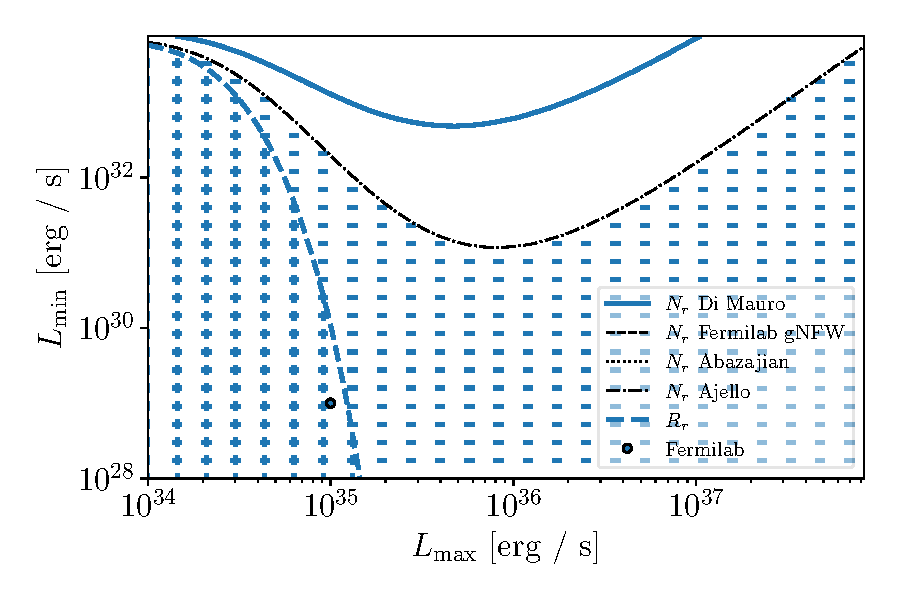
\includegraphics[width=0.49\textwidth]{figs/power-law-mult.pdf}
    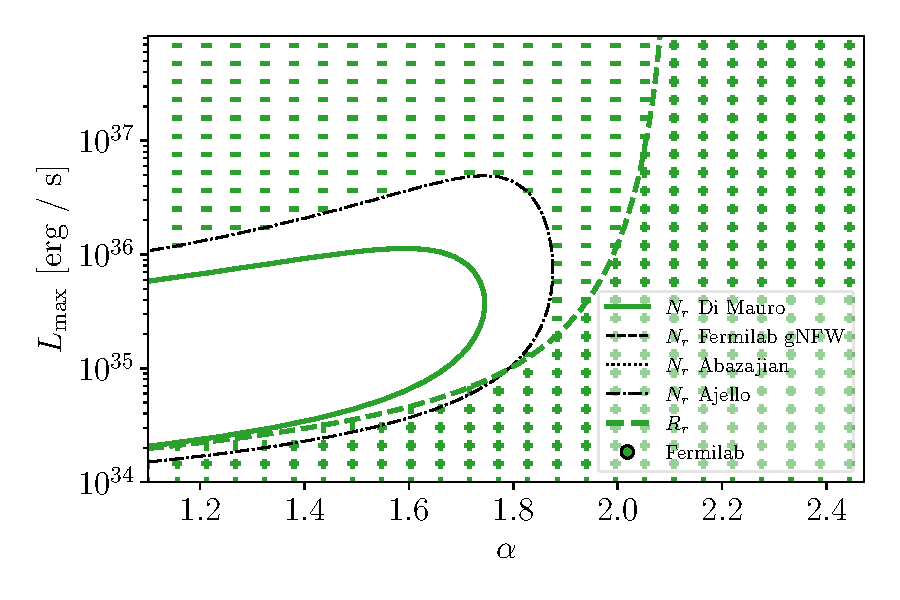
\includegraphics[width=0.49\textwidth]{figs/power-law-alpha-mult.pdf}
    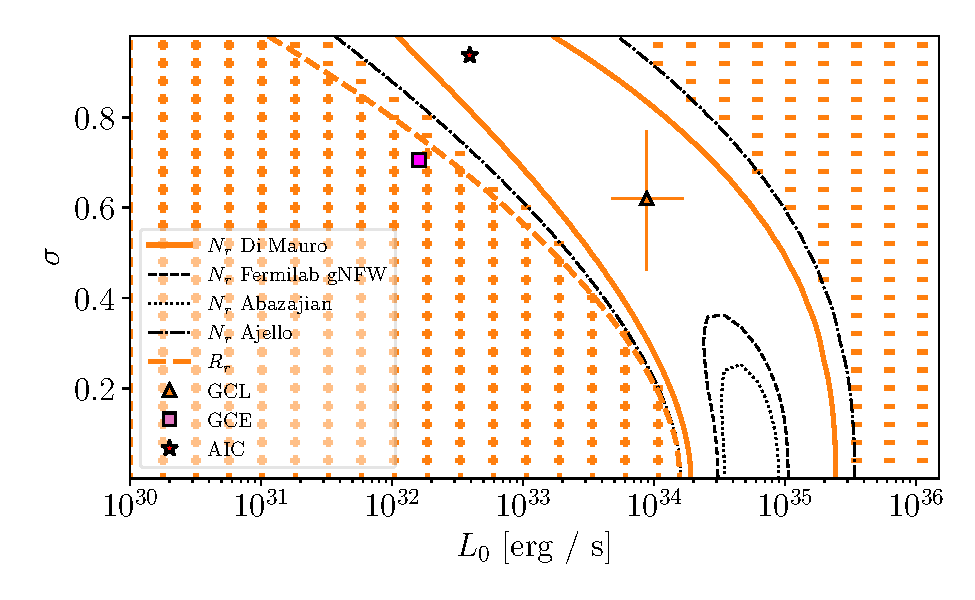
\includegraphics[width=0.49\textwidth]{figs/log-normal-mult.pdf}
    \caption{$N_\text{r}$ and $R_\text{r}$ for each luminosity function, with results for $N_\text{r}=47$ constraint shown for Fermilab gNFW's, Abazajian's, and Ajello's estimates of the GCE spectrum. \comment{I need to update the legends of these plots to be consistent with the new names of the spectrum analyses.}}
    \label{fig:multiple-fluxes}
\end{figure}

\comment{It would probably be nice to have a table showing $N_\text{r}$ and $N_\text{GCE}$ as well for different values of GCE luminosity.}

\subsection{Flux distribution}
Until this point, we have compared predictions for the population of MSPs in the GC to observations only through the number and flux of resolved MSPs. We may expand this analysis by comparing the predicted flux distribution of MSPs to the observed distribution for point sources.

We obtained the fluxes of the 47 observed point sources from the 4FGL point source catalog \cite{Fermi-LAT:2019yla}. This observed flux distribution is shown as a histogram in both panels of figure \ref{fig:flux-distro}, along with the distribution when the five extra points sources are added, corresponding to those which are added when the allowed distance between a peak in the GCE template fit and a point source in the 4FGL catalog is expanded from 0.3$^\circ$ to 0.55$^\circ$ (see section \ref{sec:observables} for details).

Added to figure \ref{fig:flux-distro} is the MSP flux distribution predicted the five parameterizations of the luminosity functions we study. Figure \ref{fig:flux-distro-fix-count} fixes the number of observed MSPs at 47 and allows the flux of the GCE to vary, and figure \ref{fig:flux-distro-fix-flux} requires each model to reproduce the flux of the GCE. Both figures are calculated with the position-dependent sensitivity model. In figure \ref{fig:flux-distro-fix-flux}, the flux distribution resulting from the step function sensitivity model is also displayed.

\begin{figure}
    \centering
    \begin{subfigure}[b]{0.47\textwidth}
        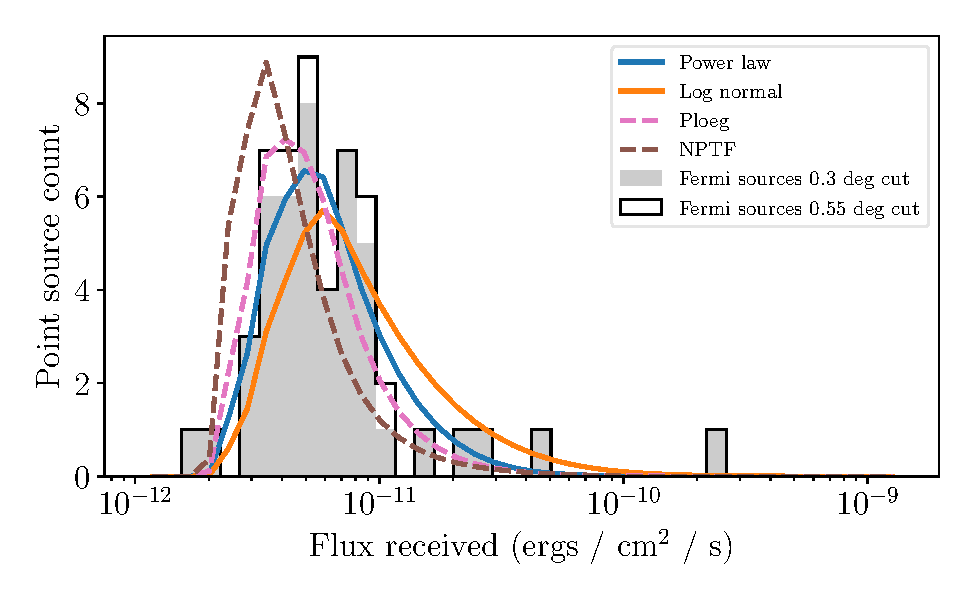
\includegraphics[width=\textwidth]{figs/flux-distro-fix-count.pdf}
        \caption{Each luminosity function is forced to reproduce 47 sources, which is the observed number}
        \label{fig:flux-distro-fix-count}
    \end{subfigure}
    \hfill
    \begin{subfigure}[b]{0.47\textwidth}
        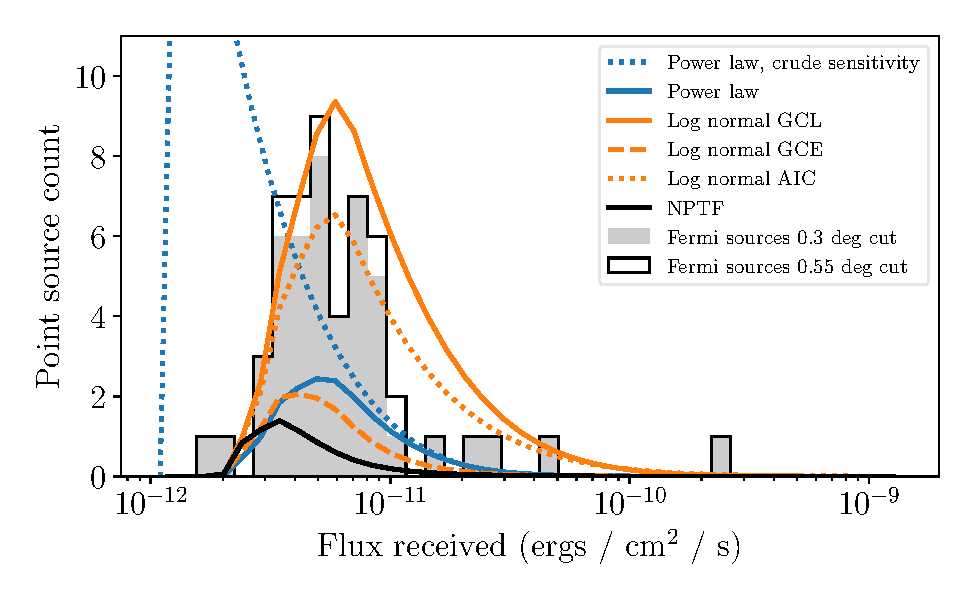
\includegraphics[width=\textwidth]{figs/flux-distro-fix-flux.pdf}
        \caption{Each luminosity function is forced to reproduce the flux of the GCE}
        \label{fig:flux-distro-fix-flux}
    \end{subfigure}
    \caption{Distribution of resolved sources predicted by each luminosity function compared to observed distribution, where observed point sources are allowed to be within 0.3$^\circ$ of spatial peaks in the GCE flux (gray histogram) and 0.53$^\circ$ (black histogram).}
    \label{fig:flux-distro}
\end{figure}

For the case when the number of observed MSPs is fixed at 47, the resultant flux of the GCE is presented in table \ref{tab:rescaled-gce-flux} and compared to the observed GCE flux.

\begin{table}
    \centering
    \begin{tabular} {|l|c|c|}
        \hline
        Luminosity function & $F_\text{GCE}^{(47)}\ (\SI{}{\erg\per\second})$ & $F^{(47)}_\text{GCE} / F^\text{obs}_\text{GCE}$\\ \hline \hline
        Power law & $\num{3.49e-09}$ & $\num{2.69}$\\
        Log normal GCL & $\num{7.91e-10}$ & $\num{0.61}$ \\
        Log normal GCE & $\num{4.57e-09}$ & $\num{3.60}$\\
        Log normal AIC & $\num{1.10e-9}$ & $\num{0.85}$ \\
        NPTF & $\num{8.29e-09}$ & $\num{6.40}$\\
        \hline
    \end{tabular}
    \caption{Total GCE flux ($F_\text{GCE}^{(47)}$) required by each luminosity function to yield 47 observed forces, and the ratio of that flux to the observed GCE flux $F_\text{GCE}^\text{obs}$ for comparison.}
    \label{tab:rescaled-gce-flux}
\end{table}





\section{Discussion}

\subsection{Sensitivity models}
Figure \ref{fig:step-and-pos} and table \ref{tab:specific-results} both demonstrate that the step function and position-dependent sensitivity models yield starkly different observables. The regions of allowed parameterization differ greatly, especially in the power law case, between the two models, and predictions for $N_\text{r}$ can differ by as much as a factor of ten for specific parameterizations. Predictions by $R_\text{r}$ differ by as much as a factor of three. This is in part because bright pulsars distant from Earth have lower flux, and therefore can appear unresolved in the position-dependent sensitivity model, but the step function sensitivity model always marks these pulsars as unresolved. The difference is also caused by the fact that lower sensitivity is correlated with MSP population density, a fact not appreciated by the step function model. The GCE log normal luminosity function differs most between sensitivity models, most likely due to \comment{its thinness and low mean, but I need to think more about exactly why this is.}

Finally, the step function threshold $L_\text{th}=\SI{e34}{\erg\per\second}$ used in ref. \cite{Zhong:2019ycb} may be unphysically low; using the conversion between flux and luminosity outlined in appendix \ref{app:lum-to-flux}, the lowest value in \textit{Fermi}'s sensitivity map corresponds to a luminosity of $\SI{1.7e34}{\erg\per\second}$. Ref. \cite{Zhong:2019ycb} also uses a threshold of $L_\text{th}=\SI{3e34}{\erg\per\second}$ sometimes, to account for the strong dependence on the value of $L_\text{th}$. \comment{They don't actually say why they use 3e34. Is it fair to put words in their mouth? Also, maybe I should use 3e34. It wouldn't actually be that hard.}

In contrast, the smoothed sensitivity model does not appear to differ from the position-dependent sensitivity model by nearly as much. \comment{Except the power law, which may be a bug? I just checked; I don't think it's a bug.} This is likely because the smoothed sensitivity model differs from the position dependent model only for MSPs near $F_\text{th}(\ell, b)$, which is a relatively small number of MSPs for most luminosity functions. Motivated by this similarity and the greater computational complexity of the smoothed sensitivity model, we will mostly use the position-dependent sensitivity model throughout the rest of this study.


\subsection{Allowed luminosity function parameterizations}
Figure \ref{fig:step-function} shows that the power law parameterization used by ref. \cite{Zhong:2019ycb}, which matches both $N_\text{r}=47$ and $R_\text{r}=0.2$ exactly when their GCE luminosity and the step function model is used, does not match the number constraint when di Mauro's GCE flux is used. When the position dependent sensitivity model is used, the constraints change so drastically that the point now produces 17.6 resolvable MSPs instead of 47 (table \ref{tab:specific-results}). The implicit uncertainty on this point, induced by uncertainties in the sensitivity model, the GCE luminosity, and observations, are therefore very large.

Figure \ref{fig:step-and-pos} also demonstrates that the GCL and AIC parameterizations of the log normal do not match observations, regardless of which sensitivity model is used. However, \ref{fig:multiple-fluxes} demonstrates that this exclusion is sensitive to the flux of the GCE used; by using a small enough flux, almost all parameterizations of the log normal luminosity function fit observations.

The fact that the GCL and AIC luminosity functions obey the number constraint when a different GCE flux is used does not necessarily mean that they are good candidates for an MSP population in the GC. The flux ratio constraint $R_\text{r}$ does not change when a different GCE flux is used, so the luminosity functions still do not match the $R_\text{r}$ constraint. Furthermore, the $R_\text{r}$ constraint has been shown above to be less dependent on the sensitivity model used, indicating that it is a more reliable constraint. The good agreement between the observed flux distribution of point sources and the predicted flux distribution of MSPs (discussed more below) also strengthens this point.

The only luminosity function that reliably matches observations is the GCE luminosity function, which was expected given that that it is the only luminosity function considered in this paper which was obtained by a fit to GCE data. This strengthens the point made by others \cite{citation-needed} that an MSP population that explains the GCE would have to have different properties than GCL MSPs. Specifically, it appears they would have to have lower luminosity or form a more peaked distribution, so that they stay in the lower left triangle of the bottom row plots of figure \ref{fig:step-and-pos}.

\subsection{Number of MSPs in the GCE}
Reference \cite{Zhong:2019ycb} determined that about three million MSPs are required to reproduce the GCE. Using a different spectrum for the GCE, that number inflates to 8 million (table \ref{tab:specific-results}). However, if a different sensitivity model is used, the region of parameterizations allowed by observational constraints can produce only thousands of MSPs (figure \ref{fig:position-dependent}).

The log normal case also produces a few thousand MSPs, while the GCE parameterization, which agrees with observational constraints, produces about 20,000 MSPs.The NPTF luminosity function also produces a few thousand MSPs. Indeed, all the specific parameterizations we studied in table \ref{tab:specific-results} result in fewer than 30,000 MSPs except for the power law luminosity function. \comment{In consultation with Tracy, make some final judgment about how many pulsars are likely to be in the GCE.}


\subsection{Flux distribution}
Our predictions of MSP flux distribution match the shape of the observed flux distribution of point sources well (fig. \ref{fig:flux-distro-fix-count}), especially for the log normal and power law luminosity functions. \comment{Should I make some Poissonian error bars and find a p value?}. However, since all luminosity functions tested match the observed flux distribution well, the flux distribution appears to be controlled by the shape of the GCE and the sensitivity model rather than the luminosity function parameterization, indicating that the observed flux distribution is unlikely to shed much light on the luminosity function of GCE MSPs. \comment{Is that too unsubstantiated to say?} Figure \ref{fig:flux-distro-fix-flux} shows that the flux distribution for the step function sensitivity model does not match the observed flux distribution in shape, since it predicts a sharp cutoff of point source detection at \textit{Fermi}'s luminosity threshold, which is not observed.





\section{Future Sensitivity}
In this section, we determine the capability of an improved $\gamma$-ray telescope to constrain the luminosity function parameters of an MSP population in the GC. We simulate an increase in sensitivity of GCE measurements by reusing the same $F_\text{th}(\ell, b)$ sensitivity map (figure \ref{fig:sensitivity}) as the one provided by the Fermi-LAT team, but with an overall multiplicative decrease. In particular, we study cases where the sensitivity is decreased by a factor of two, five, and ten and reproduce the analysis described earlier in the paper.

Plots of $N_\text{r}$, $R_\text{r}$, and $N_\text{GCE}$ for different parameterizations of the power law and log normal luminosity functions are shown in figure \ref{fig:sensitivity-results}, and values for $N_\text{r}$ and $R_\text{r}$ for specific parameterizations are given in table \ref{tab:sensitivity-values}. The number of sources in the GCE does not depend on the telescope's sensitivity, so $N_\text{GCE}$ is not included in table \ref{tab:sensitivity-values} and is only included in fig. \ref{fig:sensitivity-results} for reference. \comment{That means that the backgrounds of the column plots do not change from plot to plot. I could put them all on the same axes.}

\comment{It's difficult to draw conclusions from these plots because if you increase sensitivity, the number of observed sources will obviously change. Maybe I should be doing a different kind of analysis? Or figure out a better way to phrase things} The power law is shown to react most to changes in sensitivity level, and for both luminosity functions, the number constraint is more dependent on sensitivity than the flux ratio constraint.

\begin{figure}
    \centering
    \begin{subfigure}[b]{0.32\textwidth}
        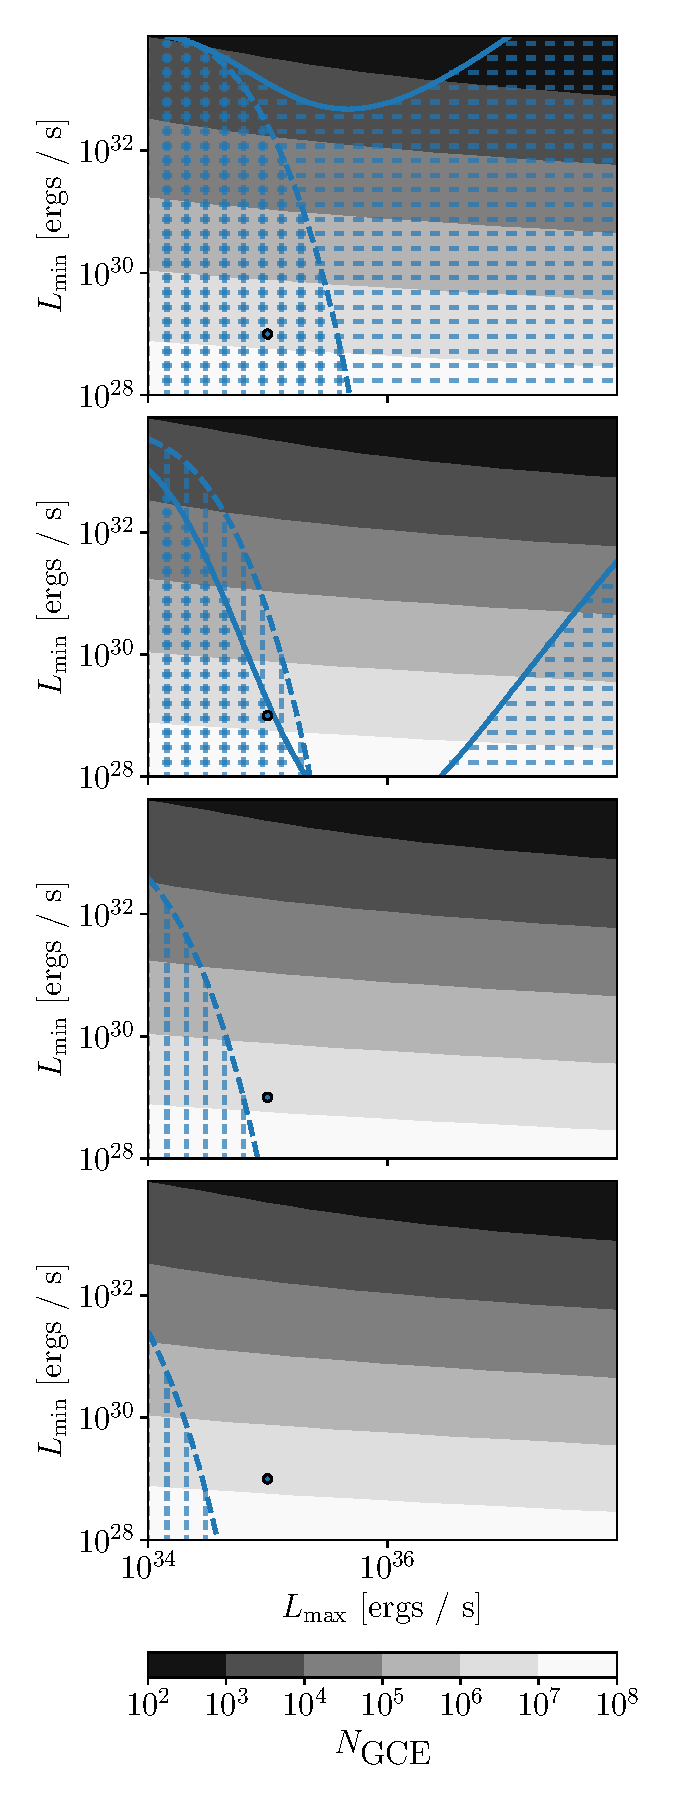
\includegraphics[width=\textwidth]{figs/power-law-sensitivity.pdf}
        \caption{Power law luminosity function varying $L_\text{min}$, $L_\text{max}$}
    \end{subfigure}
    \hfill
    \begin{subfigure}[b]{0.32\textwidth}
        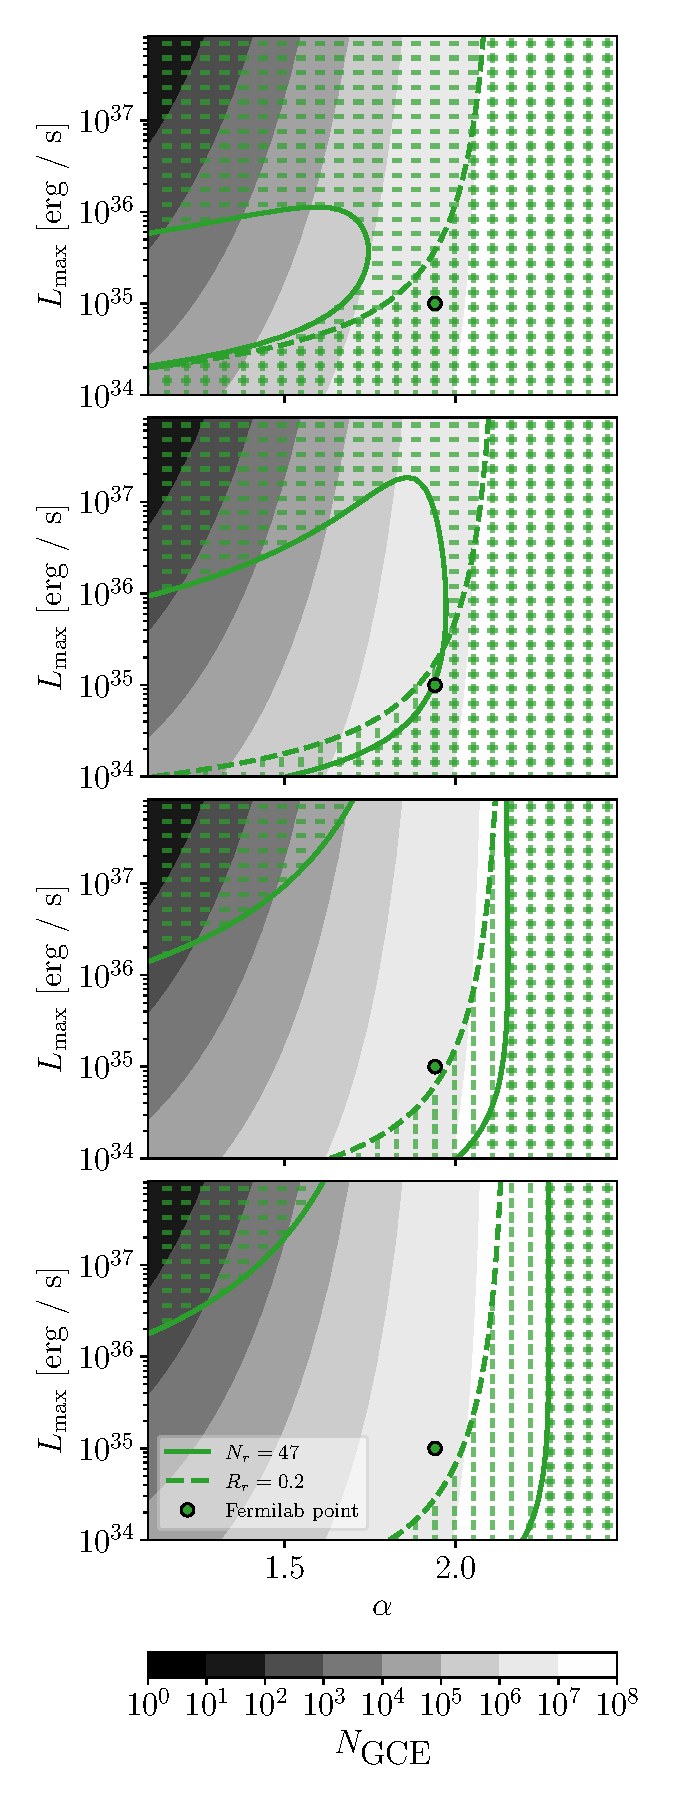
\includegraphics[width=\textwidth]{figs/power-law-alpha-sensitivity.pdf}
        \caption{Power law luminosity function varying $\alpha$, $L_\text{max}$}
    \end{subfigure}
    \hfill
    \begin{subfigure}[b]{0.32\textwidth}
        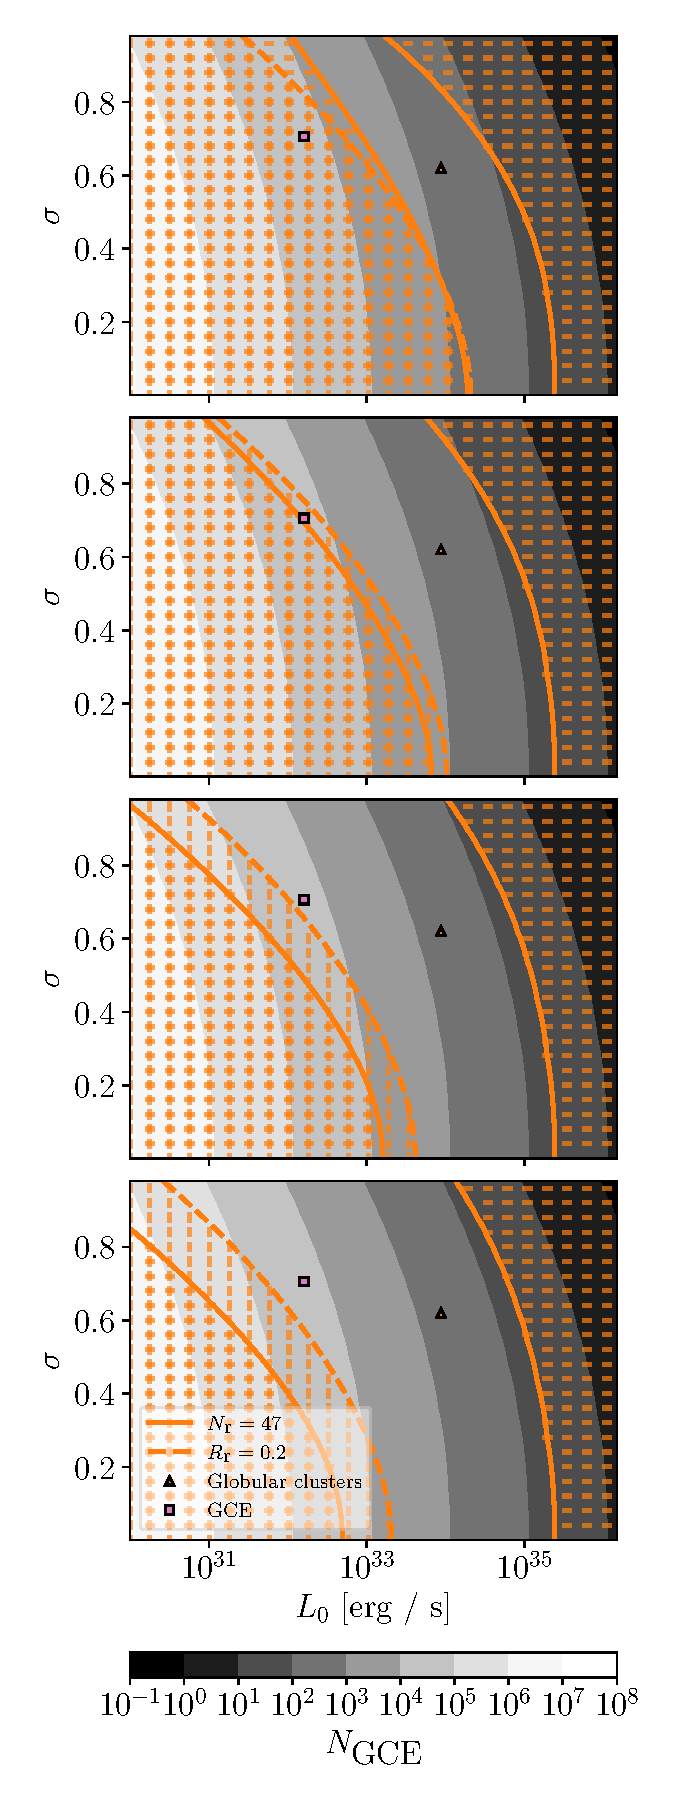
\includegraphics[width=\textwidth]{figs/log-normal-sensitivity.pdf}
        \caption{Log normal luminosity function }
    \end{subfigure}
    \caption{$N_\text{r}$, $R_\text{r}$, and $N_\text{GCE}$ for power law and log normal luminosity function parameterizations, simulating improved $\gamma$-ray telescope sensitivity, with regions allowed by the current observations of $N_\text{r}\leq 47$ and $R_\text{r} \leq 0.2$ marked with \texttt{+} symbols. The top row indicates \textit{Fermi}'s current sensitivity, while the lower rows are an overall decrease in threshold $F_\text{th}(\ell, b)$ by a factor of two, five, and ten respectively. $N_\text{GCE}$ does not depend on sensitivity but is displayed for reference.}
    \label{fig:sensitivity-results}
\end{figure}

\begin{table}
    \centering
    \begin{tabular}{|l | c c | c c | c c | c c |}
        \hline
        Luminosity function & $N_\text{r}^{\times 1}$ & $R_\text{r}^{\times 1}$ & $N_\text{r}^{\times 2}$ & $R_\text{r}^{\times 2}$ & $N_\text{r}^{\times 5}$ & $R_\text{r}^{\times 5}$ & $N_\text{r}^{\times 10}$ & $R_\text{r}^{\times 10}$\\ \hline \hline
        Power law & 17.6 & 0.101 & 45.8 & 0.157 & 137 & 0.237 & 290 & 0.298 \\
        Log normal, GCL & 77.5 & 0.692 & 142 & 0.831 & 251 & 0.941 & 331 & 0.979 \\
        Log normal, GCE & 13.4 & 0.0648 & 48.9 & 0.129 & 222 & 0.270 & 599 & 0.416  \\
        Log normal, AIC & 55.6 & 0.552 & 113 & 0.670 & 256 & 0.803 & 432 & 0.878  \\
        NFW NPTF & 7.48 & 0.0300 & 50.7 & 0.0920 & 574 & 0.480 & $\num{1.40e3}$ & 0.879 \\
        DISK NPTF & 71.7 & 0.757 & 110 & 0.839 & 180 & 0.907 & 252 & 0.939 \\
        \hline
    \end{tabular}
    \caption{Number of resolved MSPs and ratio of resolved flux to total flux based on six luminosity function parameterizations and the requirement that the MSPs reproduce the entire flux of the GCE. The assumed sensitivity of the telescope, $F_\text{th}(\ell, b)$, has been varied by a factor of 1 (i.e., sensitivity is at its current value), 2, 5, and 10, with the factor of increase given as superscripts in the header. All use the position-dependent sensitivity model. For definitions of the paramterizations, see section \ref{sec:lum-funcs}. \comment{Maybe this should be a plot.}}
    \label{tab:sensitivity-values}
\end{table}


\section{Conclusion}
\comment{I thought I'd leave writing the introduction and conclusion until the rest of the paper is done, in case things change.}

\comment{Effect of our research on the predictions by Fermilab}

\comment{Number of pulsars in the GCE}

\comment{Comparison between the GCE- and GCL-derived luminosity functions and which matches observations more accurately}

\comment{The observed flux distribution matches the predicted distribution of MSPs, but is not sensitive to the luminosity function}

\comment{Future sensitivity}


\appendix
\section{Scaling of ROIs and Spectral Ranges}
\label{app:roi-rescale}
To establish a value for the total flux of the GCE, we draw on several analyses of the GCE spectrum in section \ref{sec:total-lum}. However, not all the analyses we study use the same ROI as ours. To convert between our ROI and others', we assume an NFW squared spacial distribution of MSPs in the GCE as discussed in section \ref{sec:spacial-distro}. Then we simply calculate the ratio of flux in our region of interest $F_\Omega$ to flux in another analysis's region of interest $F_{\Omega'}$ via
\begin{equation}
    \frac{F_{\Omega'}}{F_\Omega} = \brackets{\int_{\Omega'}d\Omega\int_0^\infty ds \rho_\text{NFW}^2 (r)}\brackets{\int_{\Omega}d\Omega\int_0^\infty ds \rho_\text{NFW}^2 (r)}^{-1}.
    \label{eqn:roi-conversion}
\end{equation}
Here, $s$ represents the distance between Earth and the point of integration, and $r$ represents the galactocentric distance. They are related by $r^2 = s^2 + r_c^2 - 2 s r_c \cos\ell$, where $\ell$ is the Galactic longitude and $r_c$ is the distance between Earth and the center of the Galaxy, taken here to be $\SI{8.5}{\kilo\parsec}$ to be consistent with the rest of this study.

The flux ratio as computed by equation \ref{eqn:roi-conversion} between our region and the same $40^\circ \times 40^\circ$ without the Galactic disk cutout is 1.90. Similarly, the ratio is 1.70, 1.44,1.26, 1.04, and 0.869 for a $30^\circ \times 30^\circ $, $20^\circ \times 20^\circ$, $15^\circ \times 15^\circ$, $10^\circ \times 10^\circ$, and $7^\circ \times 7^\circ$ respectively. We mention $15^\circ \times 15^\circ$ because it is the ROI used by ref. \cite{Ajello:2015kwa}, and $7^\circ \times 7^\circ$ because it is used by refs. \cite{Abazajian:2014fta} and \cite{Gordon13}.


\section{Conversion Between GCE Luminosity and Flux}
\label{app:lum-to-flux}
This analysis requires luminosity functions to be expressed as probability distributions as a function of luminosity, since they are intended to be statements solely about the GC MSP population, made without reference to the distance of observation, and therefore the flux. Yet several papers referenced in this study express luminosity functions as a function of flux. This appendix describes how the conversion to luminosity is done.

As discussed in section \ref{sec:spacial-distro}, we represent the MSP population as distributed according to an NFW squared distribution with $\gamma = 1.2$. One way to convert a function of flux to luminosity would be to simply use the luminosity function which, when integrated over the NFW squared spacial distribution, would reproduce the observed function of flux. But this method would change the functional form of the luminosity function so that, for example, a luminosity function that is log normal when written in terms of flux would no longer be log normal when written in terms of luminosity. \comment{Is it worth devoting a whole paragraph to describing something I do not intend to do? I do it to avoid confusion.}

So for this paper, we simply convert the flux value of every bin to a luminosity according to the following method. We assume that the entire population of MPSs only contains pulsars with luminosity $L$ and ask what average flux $F$ per pulsar is observed. Integrated over the region of interest $\Omega$, this yields a constant flux to luminosity ratio of
\begin{equation}
    \frac{F}{L} = \frac{1}{4\pi}\brackets{\int_{\Omega}d\Omega\int_0^\infty ds \rho_\text{NFW}^2 (r)}\brackets{\int_{\Omega}d\Omega \int_0^\infty s^2 ds \rho_\text{NFW}^2 (r)}^{-1} = \SI{1.11e-46}{\per\centi\meter\squared}.
    \label{eqn:f-to-l}
\end{equation}
Here, $s$ represents the distance from Earth to the point of integration, and $r$ represents the distance from the GC to the point of integration. They are related by the law of cosines: $r^2 = s^2 + r_c^2 - 2s r_c \cos b\cos \ell$, where $\ell$ is the Galactic longitude. The numerical value reported was computed for $r_c = \SI{8.5}{\kilo\parsec}$. It is slightly lower than the na\"ive value of $\frac{F}{L} = \frac{1}{4\pi r_c^2} = \SI{1.16e-46}{\per\centi\meter\squared}$, which assumes that all the MSPs are at the Galactic center, and therefore does not rely on a choice of $\gamma$.

\section{Calculation of photon energy}
\label{app:photon-energy}
The parameterization of the NPTF luminosity function of ref. \cite{Lee:2015fea} is given with flux units of photons per second. To convert this to luminosity via appendix \ref{app:lum-to-flux}, we need to find the energy of a single GCE photon. To do this, we fit a broken power law to the GCE spectrum found by di Mauro and described in section \ref{sec:total-lum}, defining the flux observed from photons in an energy bin of energy $E_\gamma$ and width $dE_\gamma$ as $dF = E_\gamma N(E_\gamma)dE_\gamma$. The function $E_\gamma^2 N(E_\gamma)$ is plotted in figure \ref{fig:di-mauro-example}. The average photon energy is then calculated by
\begin{equation}
    \langle E_\gamma \rangle =  \brackets{\int_{\SI{0.1}{\giga\electronvolt}}^{\SI{100}{\giga\electronvolt}} E_\gamma N(E_\gamma) dE_\gamma} \brackets{\int_{\SI{0.1}{\giga\electronvolt}}^{\SI{100}{\giga\electronvolt}} N(E_\gamma) dE_\gamma}^{-1} = \SI{1.58e-3}{\erg}.
    \label{eqn:photon-energy}
\end{equation}
However, for the conversion of the photon flux to energy flux for the NPTF luminosity function specifically, we use a spectrum extending from $\SI{1.893}{\giga\electronvolt}$ to $\SI{11.943}{\giga\electronvolt}$, which was used in the reference that derived the flux \cite{Lee:2015fea}. This yielded an energy of $\SI{5.76e-3}{\erg}$.

If the broken power law fit to the GCE spectrum proposed by Calore et al. is used, then the energy per photon over the $\SI{0.1}{\giga\electronvolt}$ to $\SI{100}{\giga\electronvolt}$ spectrum is $\SI{1.41e-3}{\erg}$. If the fit to the Zhong et al. 2020 spectrum with $\gamma=1.2$ is used, then the photon energy is $\SI{1.35e-3}{\erg}$. We see then that the photon energy, while highly sensitive to the range of spectrum used, is not very sensitive to the GCE spectrum used.



\acknowledgments
\comment{We should probably acknowledge the Fermilab team for giving us their data. Anyone else?}






% The bibliography will probably be heavily edited during typesetting.
% We'll parse it and, using the arxiv number or the journal data, will
% query inspire, trying to verify the data (this will probalby spot
% eventual typos) and retrive the document DOI and eventual errata.
% We however suggest to always provide author, title and journal data:
% in short all the informations that clearly identify a document.


\bibliographystyle{unsrt}
\bibliography{gce.bib}

\end{document}
